% define some macros:
\newcommand{\srun}{{\tt srun}}
\newcommand{\scancel}{{\tt scancel}}
\newcommand{\squeue}{{\tt squeue}}
\newcommand{\scontrol}{{\tt scontrol}}
\newcommand{\slurmctld}{{\tt slurmctld}}
\newcommand{\slurmd}{{\tt slurmd}}


\maketitle

\begin{abstract}
Simple Linux Utility for Resource Management (SLURM) is an open source,
fault-tolerant, and highly scalable cluster management and job 
scheduling system for Linux clusters of 
thousands of nodes.  Components include machine status, partition
management, job management, and scheduling modules.  The design also 
includes a scalable, general-purpose communication infrastructure.
Development will take place in four phases:  Phase I results in a solid
infrastructure;  Phase II produces a functional but limited interactive 
job initiation capability without use of the interconnect/switch; 
Phase III provides switch support and documentation; Phase IV provides 
job status, fault-tolerance, and job queuing and control through  
Livermore's Distributed Production Control System (DPCS), a meta-batch and
resource management system.
\end{abstract}

\vspace{0.25in}

%\begin{center}
%
\epsfig{file=slurm.eps,width=4in}
%\end{center}

\newpage

\section{Overview}

SLURM\footnote{A tip of the hat to Matt Groening and creators of {\em Futurama},
where Slurm is the highly addictive soda-like beverage made from worm
excrement.} (Simple Linux Utility for Resource Management) 
is a resource management 
system suitable for use on Linux clusters, large and small.  After 
surveying\cite{Jette2002} resource managers available for Linux and finding 
none that were simple, highly scalable, and portable to different cluster 
architectures and interconnects, the authors set out to design a new system.

The result is a resource management system with the following general
characteristics:

\begin{itemize}
\item {\em Simplicity}: SLURM is simple enough to allow motivated end users
to understand its source code and add functionality.  The authors will 
avoid the temptation to add features unless they are of general appeal. 

\item {\em Open Source}: SLURM is available to everyone and will remain free;
its source code is distributed under the GNU General Public License.

\item {\em Portability}: SLURM is written in the C language, with a GNU 
autoconf configuration engine.  While initially written for Linux, 
other UNIX-like operating systems should be easy porting targets.

\item {\em Interconnect independence}: Initially, SLURM supports UDP/IP based
communication and the Quadrics Elan3 interconnect.  Adding support for other
interconnects is straightforward.  Users select the supported interconnects
at compile time via GNU autoconf.

\item {\em Scalability}: SLURM is designed for scalability to clusters of
thousands of nodes.
Prototypes of SLURM components thus far developed indicate that the
controller for a cluster with 16k nodes will occupy less than 1 MB 
of memory and performance will be excellent.\footnote{It is anticipated 
that a Linux cluster of size $>1000$ nodes will be available for testing 
before the initial public release.}

\item {\em Fault tolerance}: SLURM can handle a variety of failure modes
without terminating workloads, including crashes of the node running the SLURM
controller.

\item {\em Secure}: SLURM employs crypto technology to authenticate 
users to services and services to services.  
A Kerberos v5 infrastructure can be utilized if available.
SLURM does not assume that its networks are physically secure, 
but does assume that the entire cluster is within a single 
administrative domain with a common user base across the 
entire cluster.

\item {\em System administrator friendly}: SLURM is configured with a few
simple configuration files and minimizes distributed state.  Its interfaces
are usable by scripts and its behavior is highly deterministic.

\end{itemize}

\subsection{What is SLURM?}

As a cluster resource manager, SLURM has three key functions.  First,
it allocates exclusive and/or non-exclusive access to resources (compute nodes) to users for 
some duration of time so they can perform work.  Second, it provides 
a framework for starting, executing, and monitoring work (normally a 
parallel job) on the set of allocated nodes.  Finally, it arbitrates 
conflicting requests for resources by managing a queue of pending work.

Users interact with SLURM through three command line utilities: 
{\tt srun} for submitting a job for execution and optionally controlling it
interactively; 
{\tt scancel} for early termination of a job; 
and {\tt squeue} for monitoring job queues and basic system state.

System administrators perform privileged operations through an additional
command line utility: {\tt scontrol}.

External schedulers and meta-batch systems can submit jobs to SLURM and
order its queues through an application programming interface (API).

Compute nodes simply run a {\tt slurmd} daemon (similar to a remote shell 
daemon) to export control to SLURM.  The central controller daemon,
{\tt slurmctld}, maintains the global state and directs operations.

\subsection{What SLURM is Not}

SLURM is not a sophisticated batch system.  Its default scheduler
implements First-In First-Out (FIFO) with backfill and is not 
intended to directly implement complex site policy.
SLURM does however provide a sufficiently sophisticated API for an external 
scheduler or meta-batch system to order its queues based upon site policy.

SLURM clusters are space shared with different jobs executing 
concurrently on (typically) different nodes. 
Multiple jobs may be allocated the same node(s) 
if the administrator has configured nodes for shared access and/or 
the job has requested shared resources for improved responsiveness.
SLURM does not support gang scheduling (time-slicing 
of parallel jobs). However, the explicit preemption and later resumption 
of a job under the direction of an external scheduler may be supported 
in the future. At present an external scheduler may submit, signal, hold, 
reorder and terminate jobs via the API.

SLURM is not a meta-batch system like Globus or DPCS (Distributed Production 
Control System).  SLURM supports resource management across a single cluster.

SLURM is not a comprehensive cluster administration or monitoring package.  
While SLURM knows the state of its compute nodes, it makes no attempt to put
this information to use in other ways, such as with a general purpose event
logging mechanism or a back-end database for recording historical state.
It is expected that SLURM will be deployed in a cluster with other 
tools performing these functions. 

\subsection{Architecture}


\begin{figure}[tb]
\centerline{\epsfig{file=figures/arch.eps}}
\caption{SLURM Architecture}
\label{arch}
\end{figure}

\begin{figure}[tcb]
\centerline{\epsfig{file=figures/entities.eps,scale=0.5}}
\caption{SLURM Entities}
\label{entities}
\end{figure}


As depicted in Figure~\ref{arch}, SLURM consists of a {\tt slurmd} daemon
running on each compute node, a central {\tt slurmctld} daemon running on
a management node (with optional fail-over twin), and a four command line
utilities: {\tt srun}, {\tt scancel}, {\tt squeue}, and {\tt scontrol},
which can run anywhere in the cluster.  A scalable communications library
ties these components together.

The entities managed by these SLURM daemons include {\em nodes}, the
compute resource in SLURM, {\em partitions}, which group nodes into
logical disjoint sets, {\em jobs}, or allocations of resources assigned
to a user for a specified amount of time, and {\em job steps}, which are
sets of parallel tasks within a job.  Jobs are created within partitions
until the resources (nodes) within that paritition are exhausted. Once
a job is assigned to a set of nodes, the user will be able to initiate
parallel work in the form of job steps in any configuration within the
allocation. For instance a single job step may be started which utilizes
all nodes within the job, or several job steps may each use a portion
of the allocation.

Figure~\ref{entities} further illustrates the interrelation of these
entities as they are managed by SLURM. The diagram shows a group of
compute nodes split into two partitions. Partition 1 is running one
job, with one job step utilizing the full allocation within that job.
The job in Partition 2 has only one job step using half of the original
job allocation.

\begin{figure}[tb]
\centerline{\epsfig{file=figures/slurm-arch.eps,scale=0.5}}
\caption{SLURM Architecture - Subsystems}
\label{archdetail}
\end{figure}

Figure~\ref{archdetail} exposes the subsystems that are implemented
within the {\tt slurmd} and {\tt slurmctld} daemons.  These subsystems
are explained in more detail below.

\subsubsection{Slurmd}

The {\tt slurmd} running on each compute node can be compared to a remote
shell daemon:  it waits for work, executes the work, returns status,
then waits for more work.  It also asynchronously exchanges node and job
status with the controller.  It never communicates with other compute
nodes and the only job information it has at any given time pertains to
the currently executing jobs.

{\tt slurmd} reads its configuration from a file: {\tt /etc/slurmd.conf}
and has three major components:

\begin{itemize}
\item {\em Machine and Job Status Service}:  Respond to controller 
requests for machine and job state information, and send asynchronous 
reports of some state changes (e.g. {\tt slurmd} startup) to the controller.
Job status includes CPU and real-memory consumption information for all 
processes including user processes, system daemons, and the kernel. 

\item {\em Remote Execution}: Start, monitor, and clean up after a set
of processes, typically belonging to a parallel job, as dictated by the
controller or an \srun\ or \scancel\ process. Starting a process may
include executing a prolog script, setting process limits, setting real
and effective user id, setting environment variables, setting working
directory, allocating interconnect resources, setting corefile paths,
initializing the Stream Copy Service, and managing
process groups. Terminating a process may include terminating all members
of a process group and executing an epilog script.

\item {\em Stream Copy Service}: Allow handling of stderr, stdout, and
stdin of remote tasks. Job input may be redirected from a file or files, a
\srun\ process, or /dev/null.  Job output may be saved into local files or
sent back to the \srun\ command. Regardless of the location of stdout/err,
all job output will be locally buffered to avoid blocking local tasks.

\item {\em Job Control}: Allow asynchronous interaction with the
Remote Execution environment by propagating signals or explicit job
termination requests to any set of locally managed processes.

%\item{\em Remote Execution and Job Control}:  Start, monitor, signal, 
%and clean up after a set of processes belonging to a parallel job, as
%dictated by the controller or \srun .  Starting a process may include
%executing a prolog script, setting process limits, setting real and
%effective user id, setting environment variables, setting current working
%directory, allocating interconnect resources, setting core paths, and
%managing process groups.  Terminating a process may include terminating
%all members of a process group and executing an epilog script.
%
%\item{\em Stream Copy Service}:  Allow stderr/stdout/stdin and core files
%to be copied in and out of the spool directory for a job.  In the case
%of batch jobs, this will happen during startup and cleanup only and
%will occur between the controller and {\tt slurmd}'s.  In the case of
%interactive jobs, stdout/stderr may additionally be ``carbon copied''
%to the {\tt srun} command during job execution.
%
\end{itemize}

\subsubsection{Slurmctld}

Most SLURM state information exists in the controller, {\tt slurmctld}.
When {\tt slurmctld} starts, it reads its configuration from a file: {\tt
/etc/slurmctld.conf}.  It also can read additional state information
from a checkpoint file left by a previous {\tt slurmctld}.
{\tt slurmctld} runs in either master or standby mode, depending on the
state of its fail-over twin, if any.

{\tt slurmctld} performs several tasks simultaneously:

\begin{itemize}
\item {\em Node Manager}: Monitors the state of each node in
the cluster.  It polls {\tt slurmd}'s for status periodically and
receives state change notifications from {\tt slurmd}'s asynchronously.
It insures that nodes have the prescribed configuration before being 
considered available for use.

\item {\em Partition Manager}: Groups nodes into non-overlapping sets called
{\em partitions}. Each partition can have associated with it various job
limits and access controls.  The partition manager also allocates nodes
to jobs based upon node and partition states and configurations. Requests
to initiate jobs come from the Job Manager.  {\tt scontrol} may be used
to administratively alter node and partition configurations.

\item {\em Job Manager}: Accepts user job requests and (if applicable)
places pending jobs in a priority ordered queue. By default the job
priority will be a simple age based algorithm providing FIFO ordering.
An interface is provided for an external scheduler to establish a job's
initial priority and API's are available to alter this priority through
time for customers wishing a more sophisticated scheduling algorithm.
The job manager is awakened on a periodical basis and whenever there
is a change in state that might permit a job to begin running, such
as job completion, job submission, partition {\em up} transition,
node {\em up} transition, etc.  The job manager then makes a pass
through the priority ordered job queue. The highest priority jobs 
for each partition are allocated resources as possible. As soon as an 
allocated failure occurs for any partition, no lower-priority jobs for 
that partition are considered for initiation. 
After completing the scheduling cycle, the job manager's scheduling
thread sleeps.  Once a job has been allocated resources, the job manager
transfers necessary state information to those nodes and commences
its execution.  Once executing, the job manager will monitor and record
the job's resource consumption (CPU time used, CPU time allocated, and
real memory used) in near real-time.  When the job manager detects that
all nodes associated with a job have completed their work, it initiates
cleanup and performs another scheduling cycle as described above.

%\item {\em Switch Manager}:  Monitors the state of interconnect links 
%and informs the partition manager of any compute nodes whose links
%have failed.  The switch manager can be configured to use Simple Network
%Monitoring Protocol (SNMP) to obtain link information from SNMP-capable
%network hardware.  The switch manager configuration is optional;  without
%one, SLURM simply ignores link errors.

\end{itemize}

\subsubsection{Command Line Utilities}

The command line utilities are the user interface to SLURM functionality.
They offer users access to remote execution and job control. They also 
permit administrators to dynamically change the system configuration. The 
utilities read the global configuration file -- {\tt /etc/slurm.conf} --
to determine the host and port for \slurmctld\ requests, and the port
for \slurmd\ requests. 

\begin{itemize}
\item {\tt scancel}: Cancel a running or a waiting job, subject to
authentication. This command can also be used to sent an arbitrary 
signal to all processes associated with a job on all nodes.

\item {\tt scontrol}: Perform privileged administrative commands
such as draining a node or partition in preparation for maintenance. 
It must be run as the user {\tt root}.

\item {\tt squeue}: Display the queue of running and waiting jobs. 
{\tt squeue} can also display a summary of partition and node information.

\item {\tt srun}: Allocate resources, submit jobs to the SLURM queue,
and initiate parallel tasks. Every set of executing parallel tasks will
have an associated \srun\ process which is managing them. 
Jobs may be submitted for later execution (e.g. batch), in which case 
\srun\ will terminate after job submission. 
Jobs may also be submitted for interactive execution, where \srun\ keeps 
running to shepherd the running job. In this case, 
srun negotiates connections with remote \slurmd 's for job initiation and to
get standard output and error, forward stdin\footnote{{\tt srun} command
line options select the stdin handling method such as broadcast to all
tasks, or send only to task 0.}, and respond to signals from the user.
\srun\ may also be instructed to allocate a set of resources and
spawn a shell with access to those resources.

\end{itemize}

\subsubsection{Communications Layer}

SLURM uses the LLNL developed communications library known as 
{\tt Mongo}\footnote{Identify location of Mongo documentation here}. 
{\tt Mongo}'s API closely resembles Berkeley sockets. It is built upon the UDP 
protocol with algorithms providing better performance than TCP, particularly 
in the event of high network congestion or a high failure rate in message 
transmission. 

{\em Need more details and a reference here.}

\subsubsection{Security}

SLURM has a simple security model: 
Any user of the cluster may submit parallel jobs to execute and cancel
his own jobs.  Any user may view all SLURM configuration and state
information.  Only the user {\tt root} may modify SLURM configuration or
cancel any job.  If permission to modify SLURM configuration without a
root account is required, set-uid programs may be used to grant specific
permissions to specific users.

Trust between SLURM components and utilities is established through use
of communication-layer encryption. A shared key, group accessible from
every node in the cluster, will be used to initialize the {\tt mongo}
communications layer. Only components and utilities with access to this
shared secret will be able to communicate in the SLURM world. Unprivileged
users will not have access to this key, so SLURM utilities will need to be
installed setgid. If a utility is able to communicate with another SLURM
component, the information that the utility is presenting may be trusted.

When resources are allocated to a user by the controller, a ``job 
credential'' is generated by combining the user id, the list of
resources allocated (nodes and processors per node), and the credential
lifetime. This ``job credential'' is encrypted with a \slurmctld\ private key. 
This credential is returned to the requesting agent along with the
allocation response, and must be forwarded to the remote \slurmd 's 
on job initiation. A \slurmd\ may decrypt this credential with the
\slurmctld 's public key to quickly verify that the user may access
resources on the local node. 

Both the \slurmd\ and \slurmctld\ will also support the use
of Pluggable Authentication Modules (PAM) for additional authentication on
top of communication encryption and job credentials. In particular, if a
job credential is not forwarded to \slurmd\ on a job initiation request,
\slurmd\ may fall through to a PAM module, which may authorize the request
based upon methods such as a flat list of users or an explicit request
to the SLURM controller. \slurmctld\ may use PAM modules to authenticate
users based upon UNIX passwords, Kerberos 5, or any other method that
may be represented in a PAM module.

Access to some partitions is restricted via a `` partition key''.  This may be used,
for example, to provide specific external schedulers with exclusive access
to partitions.  Individual users will not be permitted to directly submit
jobs to such a partition, which would prevent the external scheduler
from effectively managing it.  This key will be generated by \slurmctld\
and provided to user {\tt root} via API upon request.  The external scheduler,
which must run as user {\tt root} to submit jobs on the behalf of other
users, will submit jobs as the appropriate user using this `` partition key''.

\subsection{Example:  Executing a Batch Job}

A user wishes to run a job in batch mode, in which {\tt srun} will return 
immediately and the job will execute ``in the background'' when resources
are available.

The job is a two-node run of {\em mping}, a simple MPI application.
The user submits the job:
\begin{verbatim}
srun --batch --nodes 2 --nprocs 2 mping 1 1048576
\end{verbatim}

The {\tt srun} command authenticates the user to the controller and submits
the job request. 
The request includes the {\tt srun} environment, current working directory, 
and command line option information. By default, stdout and stderr are
sent to files in the current working directory and stdin is copied from
{\tt /dev/null}.

The controller consults the partition manager to test whether the job will
will ever be able to run.  If the user has requested a non-existent partition,
more nodes than are configured in the partition, a non-existent constraint, 
etc., the partition manager returns an error and the request is discarded.
The failure is reported to {\tt srun} which informs the user and exits:
\begin{verbatim}
srun: request will never run
\end{verbatim}

On successful submission, the controller assigns the job a unique 
{\em slurm id}, adds it to the job queue and returns the 
slurm id to {\tt srun}, which reports this to user and exits, returning
success to the user's shell:

\begin{verbatim}
srun: Job 42 has been submitted
\end{verbatim}

The controller awakens the job manager which tries to run
jobs starting at the head of the job queue.  It finds job {\em 42}
and makes a successful request to the partition manager to allocate 
two nodes from the default (or requested) partition: {\em dev6} and 
{\em dev7}.

The job manager then sends a request to the \slurmd\ on the first node 
in the job {\em dev6} to initiate a \srun\ of the user's
command line\footnote{Had the user submitted a job script, this script would
be initiated on the first node of the job}. The job manager also sends a 
copy of the environment, current working directory, stdout and stderr location,
along with any other options. Additional environment variables are appended
to the user's environment before it is sent to the remote \slurmd\ detailing
the job's resources, such as the slurm job id ({\em 42}) and the
allocated nodes ({\em dev[6-7]}).

The remote \slurmd\ establishes the new environment and executes the
job script as the submitting user. The \srun\ within the job script
detects that it is running with allocated resources from the presence
of the {\tt SLURM\_JOBID} environment variable. \srun\ connects to
\slurmctld\ to request a ``job step'' to run on all nodes of the current
job. \slurmctld\ validates the request and replies with a job credential
and switch resources. \srun\ then contacts \slurmd 's running on both
{\em dev6} and {\em dev7}, passing the job credential, environment,
current working directory, command path and arguments, and interconnect
information. The \slurmd 's verify the valid job credential, connect
stdout and stderr back to \srun , establish the environment, and execute
the command as the submitting user.

Unless instructed otherwise by the user, stdout and stderr will be
copied to files in the current working directory by \srun :

\begin{verbatim}
/path/to/cwd/slurm-42.out
/path/to/cwd/slurm-42.err
\end{verbatim}

The user may examine the output files at any time if they live
in a directory that is globally accessible. In this example
{\tt slurm-42.out} would  contain:

\begin{verbatim}
  1 pinged   0:        1 bytes      5.38 uSec     0.19 MB/s                     
  1 pinged   0:        2 bytes      5.32 uSec     0.38 MB/s                     
  1 pinged   0:        4 bytes      5.27 uSec     0.76 MB/s                     
  1 pinged   0:        8 bytes      5.39 uSec     1.48 MB/s                     
  ...
  1 pinged   0:  1048576 bytes   4682.97 uSec   223.91 MB/s              
\end{verbatim}

When the tasks complete execution \srun\ is notified by \slurmd\ of each
task's exit status. \srun\ reports job step completion to the job manager
and exits. The job manager receives an exit status for the job script
and begins cleanup. It directs the \slurmd 's formerly assigned to the
job to run the job epilog if job epilogs have been configured. Finally,
the job manager releases the resources allocated to job {\em 42}
and updates the job status to {\em complete}. The records of a job's
existence will eventually be purged.

\subsection{Example:  Executing an Interactive Job}

A user wishes to run the same job in interactive mode, in which {\tt srun}
will block while the job executes and stdout/stderr of the job will be 
copied onto stdout/stderr of {\tt srun}.

The user submits the job, this time requesting an interactive run:
\begin{verbatim}
srun --nodes 2 --nprocs 2 mping 1 1048576
\end{verbatim}

The \srun\ command authenticates the user to the controller and
makes a request for an allocation {\em and} job step. The job manager
responds with a list of nodes, a job credential, and interconnect
resources on successful allocation. If resources are not immediately
available, the request will terminate or block depending upon user
option.

If the request is successful, \srun\ forwards the job run request
to the assigned \slurmd~'s in the same manner as the \srun\ in the
batch job script. In this case, the user sees the program output on 
stdout of {\tt srun}:

\begin{verbatim}
  1 pinged   0:        1 bytes      5.38 uSec     0.19 MB/s                     
  1 pinged   0:        2 bytes      5.32 uSec     0.38 MB/s                     
  1 pinged   0:        4 bytes      5.27 uSec     0.76 MB/s                     
  1 pinged   0:        8 bytes      5.39 uSec     1.48 MB/s                     
  ...
  1 pinged   0:  1048576 bytes   4682.97 uSec   223.91 MB/s              
\end{verbatim}

When the job terminates, {\tt srun} receives an EOF on each stream and
closes it, then receives the job exit status from each {\tt slurmd}.
The \srun\ process notifies \slurmctld\ that the job is complete 
and terminates. The controller contacts all \slurmd 's allocated to the
terminating job and issues a request to run the job epilog, then releases
the job's resources.

If a signal is received by {\tt srun} while the job is executing (for example,
a SIGINT resulting from a Control-C), it is sent to each {\tt slurmd} which 
terminates the individual tasks and reports this to the job status manager,
which cleans up the job.

\section{Controller Design}

The controller is modular and multi-threaded.  Independent read
and write locks will be provided for the various data structures for
scalability.  The controller state will be saved to disk immediately
upon change for fault tolerance.  The controller  will include the
following subsystems:

\begin{itemize}
\item {\em Node Manager}: Monitors the state of each node in
the cluster.  It polls {\tt slurmd}'s for status periodically and
receives state change notifications from {\tt slurmd}'s asynchronously.
It insures that nodes have the prescribed configuration before being 
considered available for use.

\item {\em Partition Manager}: Groups nodes into non-overlapping sets called
{\em partitions}. Each partition can have associated with it various job
limits and access controls.  The partition manager also allocates nodes
to jobs based upon node and partition states and configurations. Requests
to initiate jobs come from the Job Manager.  {\tt scontrol} may be used
to administratively alter node and partition configurations.

\item {\em Job management}: Accept, initiate, monitor, delete and
otherwise manage the state of all jobs in the system. This includes
prioritizing pending work.

%\item {\em Switch management}: Perform any interconnect-related monitoring
%and control needed to run a parallel job.

\end{itemize}

Each of these subsystems is described in detail below.

\subsection{Node Management}

The node manager will monitor the state of nodes.  Node information
monitored includes:

\begin{itemize}
\item Count of processors on the node
\item Size of real memory on the node
\item Size of temporary disk storage
\item State of node (RUN, IDLE, DRAINED, etc.)
\item Weight (preference in being allocated work)
\item Feature (arbitrary description)
\item IP address
\end{itemize}

The SLURM administrator could specify a list of system node
names using a regular expression (e.g. "NodeName=linux[001-512] CPUs=4
RealMemory=1024 TmpDisk=4096 Weight=4 Feature=Linux").  These values
for CPUs, RealMemory, and TmpDisk would be considered the minimal
node configuration values which are acceptable for the node to enter
into service.  The slurmd will register whatever resources actually
exist on the node and this will be recorded by the Node Manager.
Resources will be checked on slurmd initialization and periodically
thereafter.  If a node registers with less resources than configured, it
will be placed in DOWN state and the event will be logged.  Otherwise the
actual resources reported will be recorded and possibly used as a basis 
for scheduling (e.g. if the node has more RealMemory than recorded in 
the configuration file, the actual node configuration may be used for 
determining suitability for any application, alternately the data in 
the configuration file may be used for possibly improved performance).
Note the regular expression node name syntax permits even very large
heterogeneous clusters to be described in only a few lines.  In fact,
a smaller number of unique configurations can provide SLURM with greater
efficiency in scheduling work.

The weight is used to order available nodes in assigning work to them.
In a heterogeneous cluster, more capable nodes (e.g. larger memory
or faster processors) should be assigned a larger weight.  The units
are arbitrary and should reflect the relative value of that resource.
Pending jobs will be assigned the least capable nodes (i.e. lowest
weight) which satisfy their requirements.  This will tend to leave the
more capable nodes available for those jobs requiring those capabilities.

The feature is an arbitrary string describing the node, such as
a particular software package, file system, or processor speed.
While the feature does not have a numeric value, one might include a
numeric value within the feature name (e.g. "1200MHz" or "16GB\_Swap").
If the nodes on the cluster have disjoint features (e.g. different
"shared" file systems), one should identify these as features (e.g. "FS1",
"FS2", etc.).  Programs may then specify that all nodes allocated to it
should have the same feature, but that any of the specified features is
acceptable (e.g. "Feature=FS1|FS2|FS3").

Node records are kept in an array with hash table lookup. 
If nodes are given names containing sequence numbers (e.g. "lx01", "lx02", 
etc.), the hash table will permit specific node records to be located 
very quickly and this is the recommended naming convention for larger 
clusters.

An API is available to view any of this information and to update some 
node information (e.g. state). APIs designed to return SLURM
state information will permit the specification of a time-stamp.  If the
requested data has not changed since the time-stamp provided by the
application, the application's current information need not be updated.
The API will return a brief "no\_change" response rather than returning
relatively verbose state information.
Changes in node configurations (e.g. node count, memory, etc.) or the nodes 
actually in the cluster should be reflected in the SLURM configuration 
files. Updated configuration files may be read without disrupting jobs 
that are currently executing.

\subsection{Partition Management}

The partition manager will identify groups of nodes to be used for
execution of user jobs. One might consider this the scheduling component. 
Data to be associated with a partition will include:
\begin{itemize}
\item Name
\item Access controlled by key granted to user root (to support external schedulers)
\item List of associated nodes (may use regular expression)
\item State of partition (UP or DOWN)
\item Maximum time limit for any job
\item Maximum nodes allocated to any single job
\item List of groups permitted to use the partition (defaults to ALL)
\item Shared access (YES, NO, or FORCE)
\item Default partition (if not specified in job request)
\end{itemize}

It will be possible to alter most of this data in real-time in order
to effect the scheduling of pending jobs (currently executing jobs
would continue).  This information can be confined to the SLURM control
machine for better scalability.  It would be used by the Job Manager
(and possibly an external scheduler), which either exist only on the
control machine or communicate only with the control machine. 

The nodes in a partition may be designated for exclusive or non-exclusive
use by a job.  A shared value of "YES" indicates that jobs may share nodes
upon request.  A shared value of "NO" indicates that jobs are always given
exclusive use of allocated nodes.  A shared value of "FORCE" indicates
that jobs will never be insured exclusive access to nodes, but SLURM
will initiate multiple jobs on the nodes for high system utilization
and responsiveness.  In this case, job requests for exclusive node
access will not be honored.  Non-exclusive access may negatively impact
the performance of parallel jobs or cause them to fail upon exhausting
shared resources (e.g. memory or disk space). However, shared resources
should improve overall system utilization and responsiveness. The
proper support of shared resources, including enforcement of limits on
these resources, entails a substantial amount effort which we are not
planning to address presently.  However, we have designed SLURM so as
to not preclude the addition of such a capability at a later time if
so desired.  Future enhancements could include constraining jobs to a
specific CPU count or memory size within a node, which could be used
to space-share the node.  The partition manager will allocate nodes to
pending jobs upon request by the job manager.

Submitted jobs can specify desired partition, CPU count, node count,
task count,  the need for contiguous nodes assignment, and (optionally)
an explicit list of nodes.  Nodes will be selected so as to satisfy all
job requirements.  For example a job requesting four CPUs and four nodes
will actually be allocated eight CPUs and four nodes in the case of all
nodes having two CPUs each.  The submitted job may have an associated
``partition key'', and by virtue of this can be granted access to specific partitions.
The request may also indicate node configuration constraints such as
minimum real memory or CPUs per node, required features, etc.

Nodes are selected for possible assignment to a job based upon it's
configuration requirements (e.g. partition specification, minimum memory,
temporary disk space, features, node list, etc.).  The selection is
refined by determining which nodes are up and available for use.
Groups of nodes are then considered in order of weight, with the
nodes having the minimum resources to satisfy the request preferred.
Finally the physical location of the nodes is considered.

Bit maps are used to indicate which nodes are up, idle, associated
with each partition, and associated with each unique configuration.
This technique permits scheduling decisions to normally be made by
performing a small number of tests followed by fast bit map manipulations. 
If so configured, a job's resource requirements would be compared 
against the (small number of) node configuration records, each of 
which has an associated bit map. Usable node configuration bitmaps 
would be ANDed with the selected partitions bit map ANDed with the 
UP node bit map and possibly ANDed with the IDLE node bit map. 
This method can eliminated tens of thousands of node configuration 
comparisons that would otherwise be required in large heterogeneous 
clusters.

The actual selection of nodes for allocation to a job is currently
tuned for the Quadrics interconnect.  This hardware supports hardware
message broadcast, but only if the nodes are contiguous.  If a job
is not allocated contiguous nodes, a slower software based multi-case
mechanism will be used.  Jobs will be allocated continuous nodes to the
extent possible (in fact, contiguous node allocation can be required
by a job is so specified at submission time).  If contiguous nodes
can not be allocated to a job, it will be allocated resources from
the minimum number of sets of contiguous nodes possible.  If multiple
sets of contiguous nodes can be allocated to a job, the one which most
closely fits the job's requirements will be used.  This technique will
leave the largest continuous sets of nodes intact for jobs requiring them.

The partition manager will build a list of nodes to satisfy a job's
request.  It will also cache the IP addresses of
each node and provide this information to {\tt srun} at job initiation
time for improved performance.

The failure of any node to respond to the partition manager will only
effect jobs associated with that node.  In fact, jobs may indicate they
should continue executing even if nodes allocated to it cease responding.
In this case, the job will need to provide for its own fault-tolerance.
All other jobs and nodes in the cluster will continue to operate after
a node failure.  No additional work will be allocated to the failed
node and it will be pinged periodically to determine when it has been
restored to serviced.

A sample configuration file follows.

\begin{verbatim}
# 
# Sample /etc/SLURM.conf
# Author: John Doe
# Date: 11/06/2001
#
ControlMachine=lx0001
BackupController=lx0002
#
# Node Configurations
#
NodeName=DEFAULT TmpDisk=16384
NodeName=lx[0001-0002] State=DRAINED
NodeName=lx[0003-8000] CPUs=16 RealMemory=2048 Weight=16
NodeName=lx[8001-9999] CPUs=32 RealMemory=4096 Weight=40 Feature=1200MHz
#
# Partition Configurations
#
PartitionName=DEFAULT MaxTime=30 MaxNodes=2
PartitionName=login Nodes=lx[0001-0002] State=DOWN   # Don't schedule work here
PartitionName=debug Nodes=lx[0003-0030] State=UP    Default=YES
PartitionName=class Nodes=lx[0031-0040] AllowGroups=students,teachers
PartitionName=batch Nodes=lx[0041-9999] MaxTime=UNLIMITED MaxNodes=4096 Key=YES
\end{verbatim}

\subsection{Job Manager}

There are a multitude of parameters associated with each job
\begin{itemize}
\item Job name
\item User ID
\item Job ID
\item Working Directory
\item Partition
\item Priority
\item Node constraints (processors, memory, features, etc.)
\item and many more
\end{itemize}

Job records have an associated hash table for rapidly locating 
specific records. They also have bit maps of requested and/or 
allocated nodes (as described above).

The core functions to be supported by the job manager include:
\begin{itemize}
\item Request resource request (may be queued or test for availability)
\item Reset priority of jobs (for external scheduler to order queue)
\item Status job (including node list, memory and CPU use data)
\item Signal job (send arbitrary signal to all processes associated with a job)
\item Terminate job (remove all processes)
\item Preempt/resume job  (future)
\item Checkpoint/restart job (future)
\item Change node count of running job (could fail if insufficient resources are 
available, future)
\end{itemize}

Jobs will be placed in a priority ordered queue and allocated nodes as 
selected by the Partition Manager. 
SLURM implements a very simple scheduling algorithm, namely FIFO. 
An attempt will be made to schedule pending jobs on a periodic basis
and whenever any change in job, partition, or node state might permit
the scheduling of a job.  All nodes allocated to a job will remain so
until {\em all} processes associated with that job terminate.  If a
node allocated to a job fails, the job may either continue execution or
terminate depending upon its configuration.

We are well aware this scheduling algorithm will not satisfy the needs of many
customers and provide the means for establishing other scheduling
algorithms. Before a newly arrived job is placed into the queue, it
is assigned a priority that may be established by an administrator
defined program. SLURM APIs permit an external entity to alter the
priorities of jobs at any time to re-order the queue as desired.
The Maui Scheduler\footnote{http://mauischeduler.sourceforge.net/}
is one example of an external scheduler suitable for use with SLURM.

Another scheduler that we plan to offer with SLURM is
DPCS\footnote{http://www.llnl.gov/icc/lc/dpcs/dpcs\_overview.html}.  DPCS
has flexible scheduling algorithms that suit our needs well and provides
the scalability required for this application. Most of the resource
accounting and some of the job management functions presently within
DPCS would be moved into the proposed SLURM Job Management component.
DPCS will require some modification to operate within this new, richer
environment and the DPCS Central Manager requires porting to Linux.

The DPCS writes job accounting records to Unix files. Presently, these are
moved to a machine with the Sybase database. This data can be accessed
via command-line and web interfaces with Kerberos authentication and
authorization.  We are not contemplating making this database software
available through SLURM, but might consider writing this data to an open
source database if so desired.

System specific scripts can be executed prior to the initiation of a user
job and after the termination of a user job (e.g. prolog and epilog).
These scripts are executed as user {\tt root} and can be used to establish
an appropriate environment for the user (e.g. permit logins, disable
logins, terminate "orphan" processes, etc.).  An API for all functions
would be developed initially, followed by a command-line tool utilizing
the API.

The job manager will collect resource consumption information (CPU
time used, CPU time allocated, and real memory used) associated with
a job from the slurmd daemons.  When a job approaches its time limit
(as defined by wall-clock execution time) or an imminent system shutdown
has been scheduled, the job will be terminated.  The actual termination
process is to notify slurmd daemons on nodes allocated to the job of
the termination request along with a time period in which to complete
the termination.  The slurmd job termination procedure, including job
signaling, is described in the slrumd section.

If for some reason, there are non-killable processes associated with 
the job, nodes associated with those processes will be drained and 
the other nodes relinquished for other uses.

One may think of a ``job'' as described above as an allocation of resource 
and a user script rather than a collection of parallel tasks. For that, 
the script will execute \srun\ commands to initiate the parallel tasks 
or ``job steps''. The job may include multiple job steps, executing 
sequentially and or concurrently either on separate or overlapping nodes. 
Job steps have associated with them specific nodes (some or all of those 
associated with the job), tasks, and a task distribution (cyclic or 
block) over the nodes. 

The management of job steps is considered a component of the job 
manager. Supported job step functions include:
\begin{itemize}
\item Register Job Step
\item Get Job Step Information
\item Run Job Step Request
\item Signal Job Step
\end{itemize}
Job step information includes task distribution (cyclic or block) 
across the allocated nodes, processors required per task, list of 
nodes (entire set or subset of those allocated to the job), and a 
credential used to bind communications between the tasks across 
the interconnect. The \slurmctld\ will construct this credential, 
distribute it the the relevant \slurmd\ daemons, and send it to 
the \srun\ initiating the job step.

%\subsection{Switch Manager}
%
%The switch manager would be responsible for allocating switch channels and
%assigning them to user jobs. The switch channels would be de-allocated
%upon job termination.  The slurmd (on each compute node) would provide
%user jobs with the authentication required for switch use as directed
%by the switch manager. Switch health monitoring tools will also be
%implemented in phase two. It may be desirable for the SLURM daemons
%to use the switch directly for communications, particularly for the
%movement of a large executable and/or standard input file. This option
%will be investigated in phase three.

\subsection{Fault Tolerance}

A backup {\tt slurmctld}, if one is configured, will periodically ping
the primary {\tt slurmctld}.  Should the primary {\tt slurmctld} cease
responding, the backup will load state information from the last 
{\tt slurmctld} state save, and assume control.  All {\tt slurmd} daemons
will be notify of the new controller location and be requested to upload
current state information to it.  When the primary {\tt slurmctld} is
returned to service, it will tell the backup {\tt slurmctld} to save
state and terminate.  The primary will then load state, assume control,
and notify {\tt slurmd} daemons.

SLURM utilities and the APIs will read the /etc/slrumd.conf files 
and initially try to contact the primary {\tt slurmctld}. 
Should that attempt fail, an attempt will be made to contact the 
backup {\tt slurmctld} before terminating.

\section{Slurmd}

The slurm daemon, \slurmd\, is a multi-threaded daemon for managing
user jobs and monitoring system state.  Upon initiation it will read
the /etc/slurmd.conf file, capture system state, attempt an initial
connection to the SLURM controller, and subsequently await requests.
It will service requests for system state, accounting information,
job initiation, job state, job termination, and job attachment. On the
local node it will offer an API to translate local process id's into
slurm job id's. 

It's most common action will be to report system state upon request. Upon
\slurmd\ startup and periodically thereafter, it will gather the processor
count, real memory size, and temporary disk space for the node. Should
those values change, the controller will be notified.  Another thread will
be created to capture CPU, real-memory and virtual-memory consumption from
the process table entries.  Differences in resource utilization values
from one process table snapshot to the next will be accumulated. \slurmd\ 
will insure these accumulated values are not decremented if resource
consumption for a user happens to decrease from snapshot to snapshot,
which would simply reflect the termination of one or more processes.
Both the real and virtual memory high-water marks will be recorded and
the integral of memory consumption (e.g. megabyte-hours).  Resource
consumption will be grouped by user ID and SLURM job ID (if any). Data
will be collected for system users (root, ftp, ntp, etc.) as well as
customer accounts. The intent is to capture all resource use including
kernel, idle and down time.  Upon request, the accumulated values will be
uploaded to \slurmctld\ and cleared.  

%When all processes associated
%with a SLURM job have terminated, \slurmd\ with notify the controller.
%Since multiple parallel job executions may occur from within a single
%SLURM job, \slurmd\ will not execute the epilog until requested to do so
%by the controller upon termination of all processes associated with the
%SLURM job.

\slurmd\ will accept requests from \srun\ and the controller to initiate
and terminate user jobs. The initiate job request will contain at least: 
real and effective user IDs, environment variables, working directory, task
numbers, job credential, interconnect specifications and authorization,
core paths, process limits (?), slurm id, and the command line to execute. 
\slurmd\ will execute the prolog script (if any), reset its
session ID, and then initiate the job as requested. It will record to
disk the SLURM job ID, session ID, process ID associated with each task,
and user associated with the job.  In the event of \slurmd\ failure,
this information will be recovered from disk in order to identify a
specific job. This  job identity will be used in communications with
the SLURM controller.

\marginpar{We can get this job registration and signalling 
code from DPCS. --MJ}

The job termination request will contain the SLURM job ID and a delay
period.  Jobs will have an API made available to register with \slurmd\
exactly which process(s) should be sent what signals with how much lead
time prior to termination.  \slurmd\ will send the requested signal (or
SIGNXCPU if none specified) to the identified process(es) associated with
the SLURM job (or all processes associated with that session ID or process
tree by default), sleep for the delay specified, and send SIGKILL to all
of the job's processes.  If the processes do not terminate, SIGKILL will
be sent again.  If the processes still do not terminate slurmd will notify
the slurmctld, which will log the event and set node's state to DRAINED.
After all processes terminate, slurmd will execute the epilog program
(if any).

\section{Command Line Utilities}

\subsection{scancel}

{\tt scancel} will prematurely terminate a queued or running job.
If the job is in the queue, it will just be removed.  If the job is
running, it will be signaled and terminated as described in the \slurmd\
section of this document.  It will identify the job(s) to be terminated
through input specification of: SLURM job ID or user name.  If no job
specification is supplied, the user will be asked for one.  If the user
name is supplied, all jobs associated with that user will be terminated.
{\tt scancel} can only be executed by the job's owner or user root.

\subsection{scontrol}

{\tt scontrol} is a tool meant for SLURM administration by user root. 
It provides the following capabilities:
\begin{itemize}
\item Reconfigure - Cause slurmctld to re-read its configuration file.
\item Show build parameters - Display the values of parameters that SLURM 
was built with such as locations of files and values of timers. This can 
either display the value of specific parameters or all parameters.
\item Show job state - Display the state information of a particular job 
or all jobs in the system.
\item Show job step state - Display the state information of a particular 
job step or all job steps in the system.
\item Show node state - Display the state and configuration information 
of a particular node, a set of nodes (using regular expressions to 
identify their names, or all nodes.
\item Show partition state - Display the state and configuration information 
of a particular partition or all partitions.
\item Update job state - Update the state information of a particular job 
in the system. Note that not all state information can be changed in this 
fashion (e.g. the nodes allocated to a job).
\item Update node state - Update the state of a particular node. Note that 
not all state information can be changed in this fashion (e.g. the amount 
of memory configured on a node). In some cases, you may need to modify 
the SLURM configuration file and cause it to be re-read using the "Reconfigure" 
command described above.
\item Update partition state - Update the state of a partition node. Note that 
not all state information can be changed in this fashion (e.g. the default 
partition). In some cases, you may need to modify the SLURM configuration 
file and cause it to be re-read using the "Reconfigure" command described above.
\end{itemize}

\subsection{squeue}

{\tt squeue} will report the state of SLURM jobs.  It can filter these
jobs input specification of job state (RUN, PENDING, etc.), job ID,
user name, and job name.  If no specification is supplied, the state of
all jobs will be reported.

{\tt squeue} can also report the state of SLURM partitions and nodes.  By
default, it will report a summary of partition state with node counts and
a summary of the configuration of those nodes (e.g.  "PartitionName=batch
Nodes=lx[1000-9999] RealMemory=2048-4096 IdleNodes=1234 ...").

\subsection{srun}

\srun\ is the user interface to accessing resources managed by SLURM.
Users may utilize \srun\ to allocate resources, submit batch jobs, 
run jobs interactively, and attach to currently running jobs. \srun\ 
supports a full range of options to specify job constraints and
characteristics, for example minimum real memory, temporary disk space,
and cpus per node, as well as time limits, stdin/stdout/stderr 
handling, signal handling, and working directory for job.
The full range of options are detailed in table~\ref{srun_opts}.

\begin{table}[htb]
\begin{center}
  \begin{tabular}[t]{lcl}
   \hhline{---}
      Option & Arg type & Description \\
   \hhline{---}
      {\em batch}	   & boolean& submit a batch script to job queue      \\
      {\em nprocs}         & number & number of processes to run.  	      \\
      {\em cpus-per-task } & number & number of cpus needed per process.      \\
      {\em nodes}	   & number & number of nodes on which to run.	      \\
      {\em partition}	   & string & partition name in which to run.         \\
      {\em timelimit}	   & number & wall clock timelimit for job.           \\
      {\em cddir}	   & string & working directory of remote processes   \\
      {\em immediate}	   & boolean& exit if resources are not immediately available  \\
      {\em overcommit}     & boolean& allow more than 1 process per cpu	      \\
      {\em label}	   & boolean& prepend task number to lines of stdout/err \\
      {\em distribution}   & string & distribution method for processes (block$|$cyclic) \\
      {\em job-name}	   & string & name of job 			      \\
      {\em output}         & string & location of stdout redirection	      \\
      {\em input}	   & string & location of stdin redirection	      \\
      {\em error}	   & string & location of stderr redirection	      \\
      {\em signal-opts}(?) & string & signal handling options (?)	      \\
      {\em allocate}	   & boolean& allocate nodes only		      \\
      {\em attach}	   & string & attach \srun\ to a running job	      \\
      {\em mincpus} 	   & number & minimum number of cpus per node         \\
      {\em mem}		   & number & minimum amount of real memory per node  \\
      {\em tmp}	           & number & minimum amount of temporary disk space  \\
      {\em constraint}     & string & arbitrary feature constraints	      \\
      {\em nodelist}	   & string & request a specific set of hosts	      \\
      {\em debug}	   & boolean& print debug output		      \\
      {\em verbose}	   & boolean& verbose operation			      \\
      {\em version}	   & boolean& print \srun\ version and exit	      \\
   \hhline{---}
  \end{tabular}
\caption{\label{srun_opts} \srun\ options}
\end{center}
\end{table}

The \srun\ utility can run in four different modes: {\em interactive},
in which the \srun\ process remains resident in the user's session,
manages stdout/stderr/stdin and forwards signals to the remote tasks, {\em
batch} in which \srun\ submits a job script to the SLURM queue for later
execution, {\em allocate} in which \srun\ requests resources from
the SLURM controller and spawns a shell with access to those resources,
and finally {\em attach} in which \srun\ will attach to a currently
running job and display stdout/stderr in real time from the remote tasks,
forward signals from the user's terminal and so on.

An interactive job may also be forced into the ``background'' with a
special control sequence typed at the user's terminal. This sequence will
cause another \srun\ to attach to the running job while the interactive
\srun\ terminates. Output from the running job will subsequently be
redirected to files in the current working directory and stdin will be
copied from {\tt /dev/null}. A backgrounded job may be reattached
to a user's terminal at a later time by running
\begin{verbatim}
  srun --attach jobid 
\end{verbatim}
at any time, though the remote \srun\ will not be terminated as the result 
of an attach.

\section{Job Initiation Design}

There are three modes in which jobs may be run by users under SLURM. The
first and most simple is {\em interactive} mode, in which stdout and
stderr are displayed on the user's terminal in real time, and stdin and
signals may be forwarded from the  terminal transparently to the remote
tasks. The second is {\em batch} or {queued} mode, in which the job is
queued until the request for resources can be met, at which time the
job is run by SLURM as the submitting user. In {\em allocate} mode,
a job is allocated to the requesting user, under which the user may
manually run job steps via a script or in a subshell spawned by \srun .

\begin{figure}[tb]
\centerline{\epsfig{file=figures/connections.eps,scale=0.25}}
\caption{\small Job initiation connections overview. 1. \srun\ connects to 
         \slurmctld\ requesting resources. 2. \slurmctld\ issues a response,
	 with list of nodes and job credential. 3. \srun\ opens a listen
	 port for every task in the job step, then sends a run job step
	 request to \slurmd . 4. \slurmd 's initiate job step and connect
	 back to \srun\ for stdout/err. }
\label{connections}
\end{figure}

Figure~\ref{connections} gives a high-level depiction of the connections
that will occur between SLURM components during a general interactive job
startup. \srun\ will request resources from the \slurmctld\ which will 
respond with the list of allocated nodes, timelimit, job credential, etc.
if the request is granted. \srun\ then initializes listen ports for each
task and sends a message to the \slurmd 's on the allocated nodes requesting
that the remote processes be initiated. The \slurmd 's begin execution of
the tasks and connect back to \srun\ for stdout and stderr. This process and
the other initiation modes are described in more detail below.

\subsection{Interactive job initiation}

\begin{figure}[tb]
\centerline{\epsfig{file=figures/interactive-job-init.eps,scale=0.5} }
\caption{\small Interactive job initiation. \srun\ simultaneously allocates nodes
         and a job step from \slurmctld\ then sends a run request to all
	 \slurmd 's in job. Dashed arrows indicate a periodic request that
	 may or may not occur during the lifetime of the job.}
\label{init-interactive}
\end{figure}

Interactive job initiation is illustrated in figure~\ref{init-interactive}.
The process begins with a user invoking \srun\ in interactive mode -- in 
figure~\ref{init-interactive}, the user has requested an interactive
run of the executable ``{\tt cmd}'' in the default partition. 

After processing command line options, \srun\ sends a message to
\slurmctld\ registering a job step. This message simultaneously requests
an allocation (or job) and a job step. \srun\ waits for a reply from
\slurmctld , which may not come instantly if the user has requested that
\srun\ block until resources are available. When resources are available
for the user's job, \slurmctld\ replies with a job credential, list of
nodes that were allocated, cpus per node, and so on. \srun\ then sends
a message each \slurmd\ on the allocated nodes requesting that a job
step be initiated. The \slurmd 's verify that the job is valid using
the forwarded job credential and then respond to \srun .

Each \slurmd\ invokes a job thread to handle the request, which in turn
invokes a task thread for each requested task. The task thread connects
back to a port opened by \srun\ for stdout and stderr. The host and
port for this connection is contained in the run request message sent
to this machine by \srun . Once stdout and stderr have successfully 
been connected, the task thread takes the necessary steps to initiate 
the user's executable on the node, initializing environment, current
working directory, and interconnect resources if needed. 

Once the user process exits, the task thread records the exit status and
sends a task exit message back to \srun . When all local processes
terminate, the job thread exits. The \srun\ process will either wait
for all tasks to exit, or attempt to clean up the remaining processes
when a single task exits based upon user option. Regardless, once all
tasks are finished, \srun\ sends a message to the \slurmctld\ releasing
the allocated nodes, then exits with an appropriate exit status.

When the \slurmctld\ recieves notification that \srun\ no longer needs
the allocated nodes, it issues a request for the epilog to be run on each of
the \slurmd 's in the allocation. As \slurmd 's report that the epilog ran
successfully, the nodes are returned to the partition.

\subsection{Queued (batch) job initiation}

\begin{figure}[tb]
\centerline{\epsfig{file=figures/queued-job-init.eps,scale=0.5} }
\caption{\small Queued job initiation. 
         \slurmctld\ initiates the user's job as a batch script on one node. 
	 Batch script contains an srun call which initiates parallel tasks 
	 after instantiating job step with controller. The shaded region is 
	 a compressed representation and is illustrated in more detail in the 
	 interactive diagram (figure~\ref{init-interactive}).}
\label{init-batch}
\end{figure}

Figure~\ref{init-batch} illustrates the initiation of a queued job in SLURM.
The user invokes srun in batch mode by supplying the {\tt --batch} option 
to \srun . Once user options are processed, \srun\ sends a batch job request
to \slurmctld\ that contains the input/output location for the job, current
working directory, environment, requested number of nodes, etc. The 
\slurmctld\ queues the request in its priority ordered queue. 

Once the resources are available and the job has a high enough priority,
\slurmctld\ allocates the resources to the job and contacts the first node 
of the allocation requesting that the user ``job'' be started. In this case
the job may either be another invocation of \srun\ or a {\em job script} which
has multiple invocations of \srun\ within it. The \slurmd\ on the remote
node responds to the run request, initiating the job thread, task thread, 
and user script. An \srun\ executed from within the script detects that it
has access to an allocation and initiates a job step on some or all of the
nodes within the job.

Once the job step is complete, the \srun\ in the job script notifies the
\slurmctld\, and terminates. The job script continues executing and may
initiate further job steps. Once the job script completes, the task
thread running the job script collects the exit status and sends a task exit
message to the \slurmctld . The \slurmctld\ notes that the job is complete
and requests that the job epilog be run on all nodes that were allocated.
As the \slurmd 's respond with successful completion of the epilog, 
the nodes are returned to the partition.

\subsection{Allocate mode initiation}

\begin{figure}[tb]
\centerline{\epsfig{file=figures/allocate-init.eps,scale=0.5} }
\caption{\small Job initiation in allocate mode. Resources are allocated and
         \srun\ spawns a shell with access to the resources. When user runs 
	 an \srun\ from within the shell, the a job step is initiated under
	 the allocation.}
\label{init-allocate}
\end{figure}

In allocate mode, the user wishes to allocate a job and interactively run
job steps under that allocation. The process of initiation in this mode
is illustrated in figure~\ref{init-allocate}. The invoked \srun\ sends
an allocate request to \slurmctld , which, if resources are available,
responds with a list of nodes allocated, time limit, etc. The \srun\
process spawns a shell on the user's terminal with access to the
allocation,  then waits for the shell to exit (at which time the job
will be considered complete). 

An \srun\ initiated within the allocate subshell will recognize that it
is running under an allocation and therefore already within a job. Provided
with no other arguments, \srun\ started in this manner will initiate a job
step on all nodes within the current job. However, the user may select
a subset of these nodes implicitly by using the \srun\ {\tt --nodes}  
option, or explicitly by specifying a relative nodelist 
( {\tt --nodelist=[0-5]} ). 

An \srun\ executed from the subshell will read the environment and
user options, then notify the controller that it is starting a job step
under the current job. The \slurmctld\ registers the job step and responds
with a job credential. \srun\ then initiates the job step using the same
general method as described in the section on interactive job initiation.

When the user exits the allocate subshell, the original \srun\ recieves
exit status, notifies \slurmctld\ that the job is complete, and exits. 
The controller runs the epilog on each of the allocated nodes, returning
nodes to the partition as they complete the epilog.


\section{Infrastructure: Communications Library}

\begin{figure}[htb]
\centerline{\epsfig{file=LCM.communicate.eps,scale=0.5}}
\caption{Sample communications with fanout = 2}
\label{communicate}
\end{figure}
Optimal communications performance will depend upon hierarchical communications
patterned after DPCS and GangLL work. The SLURM control machine will generate a
list of nodes for each communication. The message will then be sent to one of
the nodes. 
The daemon on that node receiving the message will divide the node list into
two or more new lists of similar size and retransmit the message to one node on
each list. Figure~\ref{communicate} shows the communications for a fan-out of 
two.  Acknowledgments will optionally be sent for the messages to confirm 
receipt with a third message to commit the action. Our design permits the 
control machine to delegate one or more compute machine daemons as responsible 
for fault-tolerance, collection of acknowledgment messages, and the commit
decision. This design minimizes the control machine overhead for performance
reasons. This design also offers excellent scalability and fault 
tolerance.\footnote{Arguments to the communications request include:
\begin{itemize}
\item Request ID
\item Request (command or acknowledgment or commit)
\item List of nodes to be effected
\item Fan-out (count)
\item Commit of request to be required (Yes or No or Delegate node receiving
      message) 
\item Acknowledgment requested to node (name of node or NULL)
\item Acknowledgment requested to port (number)
\end{itemize} }

Security will be provided by the use of reserved ports, which must be opened by
root-level processes. SLURM daemons will open these ports and all user requests
will be processed through those daemons. 

\subsection{Infrastructure: Other}

The state of slurmctld will be written periodically to disk for
fault tolerance. Daemons will be initiated via {\tt inittab} using 
the {\tt respawn} option to insure their continuous execution. 
If the control machine itself becomes inoperative, its functions can
easily be moved in an automated fashion to another computer. In fact, the
computer designated as alternative control machine can easily be relocated as
the workload on the compute nodes changes. The communications library design is
very important in providing this flexibility.

A single machine will serve as a centralized cluster manager and database. We
do not anticipate user applications executing on this machine. 

The syslog tools will be used for logging purposes and take advantage of the 
severity level parameter.

\section{Development Plan}

The design calls for a four-phase development process.  Phase one will
develop infrastructure: the communications layer, node status information 
collection and management.  There will be no development of a scheduler 
in phase one.

Phase two will provide basic job management functionality:  basic job and 
partition management plus simple scheduling, but without use of an
interconnect. 

Phase three will add Quadrics Elan3 switch support and overall documentation.  

Phase four rounds out SLURM with job accounting, fault-tolerance, 
and full integration with DPCS (Distributed Production Control System).

\appendix
\newpage

\section{Glossary}

\begin{description}
\item[DCE]	Distributed Computing Environment
\item[DFS]	Distributed File System (part of DCE)
\item[DPCS]	Distributed Production Control System, a meta-batch system 
		and resource manager developed by LLNL
\item[GangLL]	Gang Scheduling version of LoadLeveler, a joint development 
		project with IBM and LLNL
\item[Globus]	Grid scheduling infrastructure
\item[Kerberos]	Authentication mechanism
\item[LoadLeveler] IBM's parallel job management system
\item[LLNL]	Lawrence Livermore National Laboratory
\item[NQS]	Network Queuing System (a batch system)
\item[OSCAR]	Open Source Cluster Application Resource
\end{description}

\newpage
\bibliographystyle{plain}
\bibliography{project}
